\documentclass[10pt,dvipdfmx]{jsarticle}
\usepackage{ascmac}
\usepackage[margin=15truemm]{geometry}
\usepackage{amsmath}
\usepackage[dvipdfmx]{graphicx}
\usepackage{subcaption}
\setlength{\columnseprule}{0.3mm}


\begin{document}

\title{信号処理特論 第14回課題}
\author{視覚認知システム研究室\\学籍番号:2433730032 岡村 翼}
\date{\today}
\maketitle

{\textgt{課題5} }
「信号処理」のプリントの課題5でDFTを用いて\\
(1)出力応答の予測\\
(2)システム同定\\
(3)逆畳込み\\
について、それぞれ真値のy(n), g(n), x(n)と比較する.\\

(1),(2),(3)について真値と推定値を比較したものを図\ref{fig:comparison}に示す.\\

\begin{figure}[h]
    \centering
    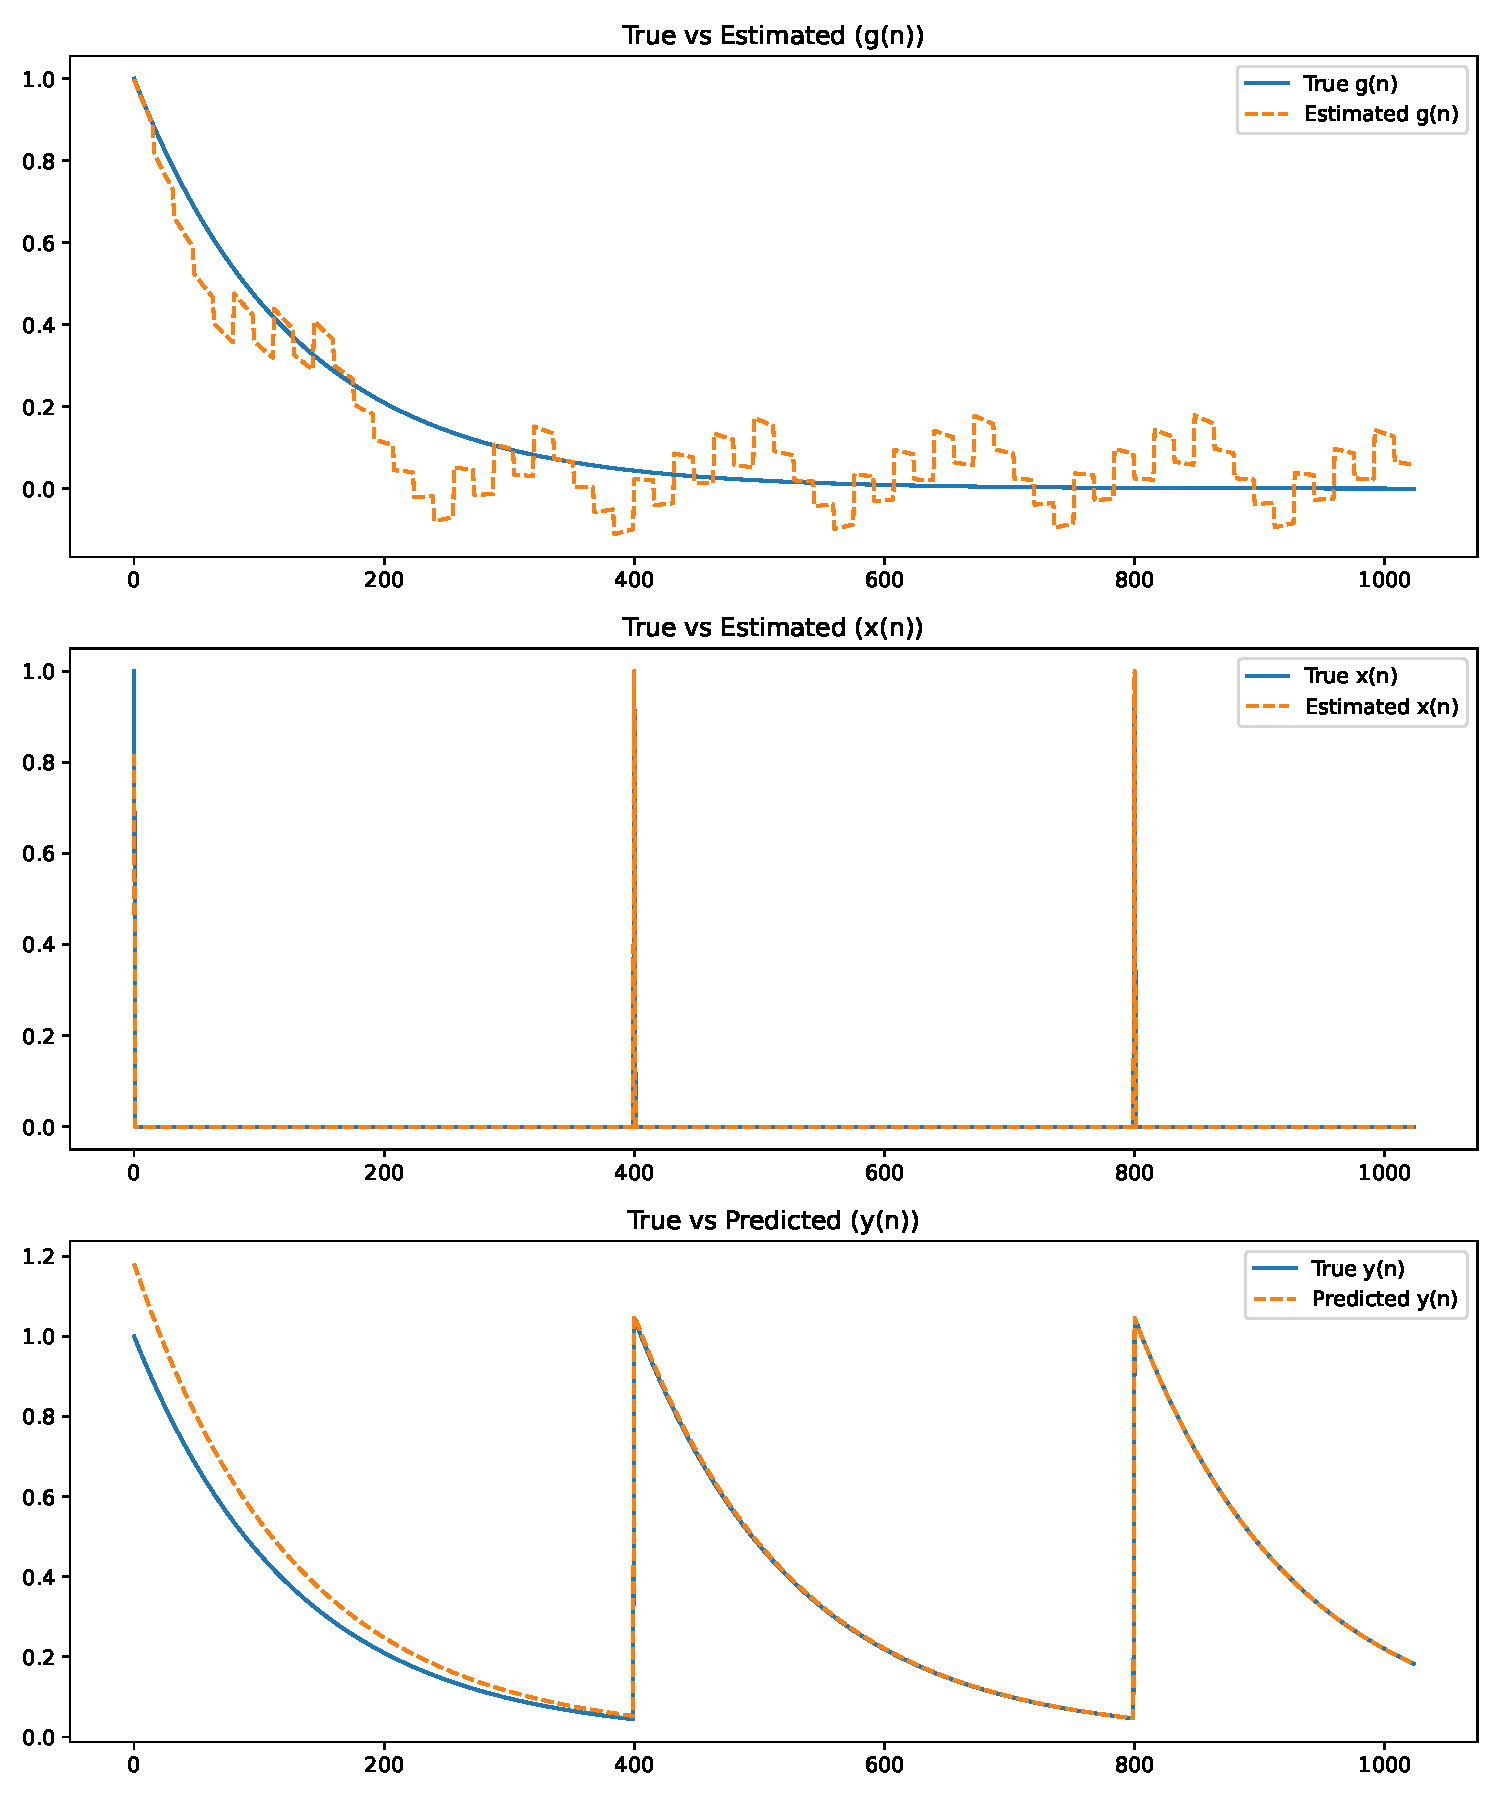
\includegraphics[width=0.8\textwidth]{comparison.pdf}
    \caption{DFTcomparison}
    \label{fig:comparison}
\end{figure}

 図\ref{fig:comparison}より、x(n)とy(n)についてはnの増加とともに推定値の精度が上昇し、n=250程度で真値と同程度の値になった.\\
 しかし、g(n)については推定値が真値付近で安定せず、予測が困難であった.

\end{document}